\section{Introduction}
Begin with the positive integers and remove multiples of prime numbers one prime at a time. At a stage headed by the prime $p$, the accepted values are precisely the integers not divisible by any prime smaller than $p$. These survivors repeat periodically. If $e_i$ and $e_{i+1}$ are consecutive survivors, then $e_{i+1}-e_i$ is their gap; the gaps across one complete period form a finite cycle.
This periodic accepted-value object is the \textbf{Sieve Sequence}, introduced and formally verified in \href{https://github.com/thiagomata/prime-numbers/blob/master/articles/chapter6/sieve-sequence.md}{Formal Verification of Sieve Sequence Stages and Their Transitions} \cite{sievesequence2026}; its finite gap cycle is the representation used throughout this article.
After multiples of $2$ have been removed, every survivor is odd. Every gap is therefore even, and $2$ is the smallest possible gap. A \textbf{2-gap} is a pair of consecutive survivors $x$ and $x+2$. At the stage headed by a prime $Q$, all primes below $Q$ have been installed as filters. A surviving 2-gap whose endpoints lie in the square-safe window $[Q,Q^2)$ is therefore a twin-prime pair: any composite number below $Q^2$ has a prime divisor below $Q$ and would already have been removed.
When the sieve later reaches the stage headed by $x$, the same pair appears as the first gap after the head. Infinitely many such head 2-gaps would give infinitely many twin-prime pairs. But survival can be asked at three different spatial scales:
1. some 2-gap exists somewhere in the complete period at every layer; 2. a 2-gap occurs in each sufficiently large square-safe window; or 3. the first gap after the distinguished head equals $2$ infinitely often.
The first statement is global and purely combinatorial. The second is local but benefits from a window whose length grows quadratically. The third concerns one position and therefore has no window-size reserve. Mixing these meanings hides the actual threshold.
The following two empirical views make the distinction visible in the deterministic Sieve Sequence. They use the same 200 stages and the same 2-focused compression: every 2-gap receives its own green cell, while each maximal run of consecutive non-2 gaps is collapsed into one colored cell equal to its sum. An internal colored cell therefore measures the total distance between two consecutive 2-gaps. Both views display $1{,}400$ compressed units from every row; they differ only in where those rows are placed horizontally.
\textbf{View A — independent compressed snapshots.} Every row begins at column zero, so its horizontal coordinate counts compressed units from that stage's own head. This is the original view. It honestly shows the texture within each stage, but its curved or noisy-looking vertical drift must not be read as a 2-gap changing before the square boundary: equal columns in adjacent rows need not represent the same surviving values.
\begin{figure}[htbp]
\centering

\includegraphics[width=\textwidth]{figures/gap-heatmap-2focused.pdf}
\caption{Independent 2-focused snapshots of 200 Sieve Sequence stages: every row restarts at its own head}
\end{figure}
\textbf{View B — shared-safe-2 alignment.} For each pair of adjacent rows, let $h$ be the previous stage's head. A safe anchor is a 2-gap with the same raw starting value in both rows and with both endpoints strictly below $h^2$. The alignment calculation compares the compressed indices of every such shared safe 2-gap and shifts the later row by their common difference. Across the 199 observed transitions, the 200-stage dataset exhibits 118 differences of zero and 81 of one; every safe anchor within each transition agrees with that row's difference. Accumulating those differences produces the alternative view below.
\begin{figure}[htbp]
\centering
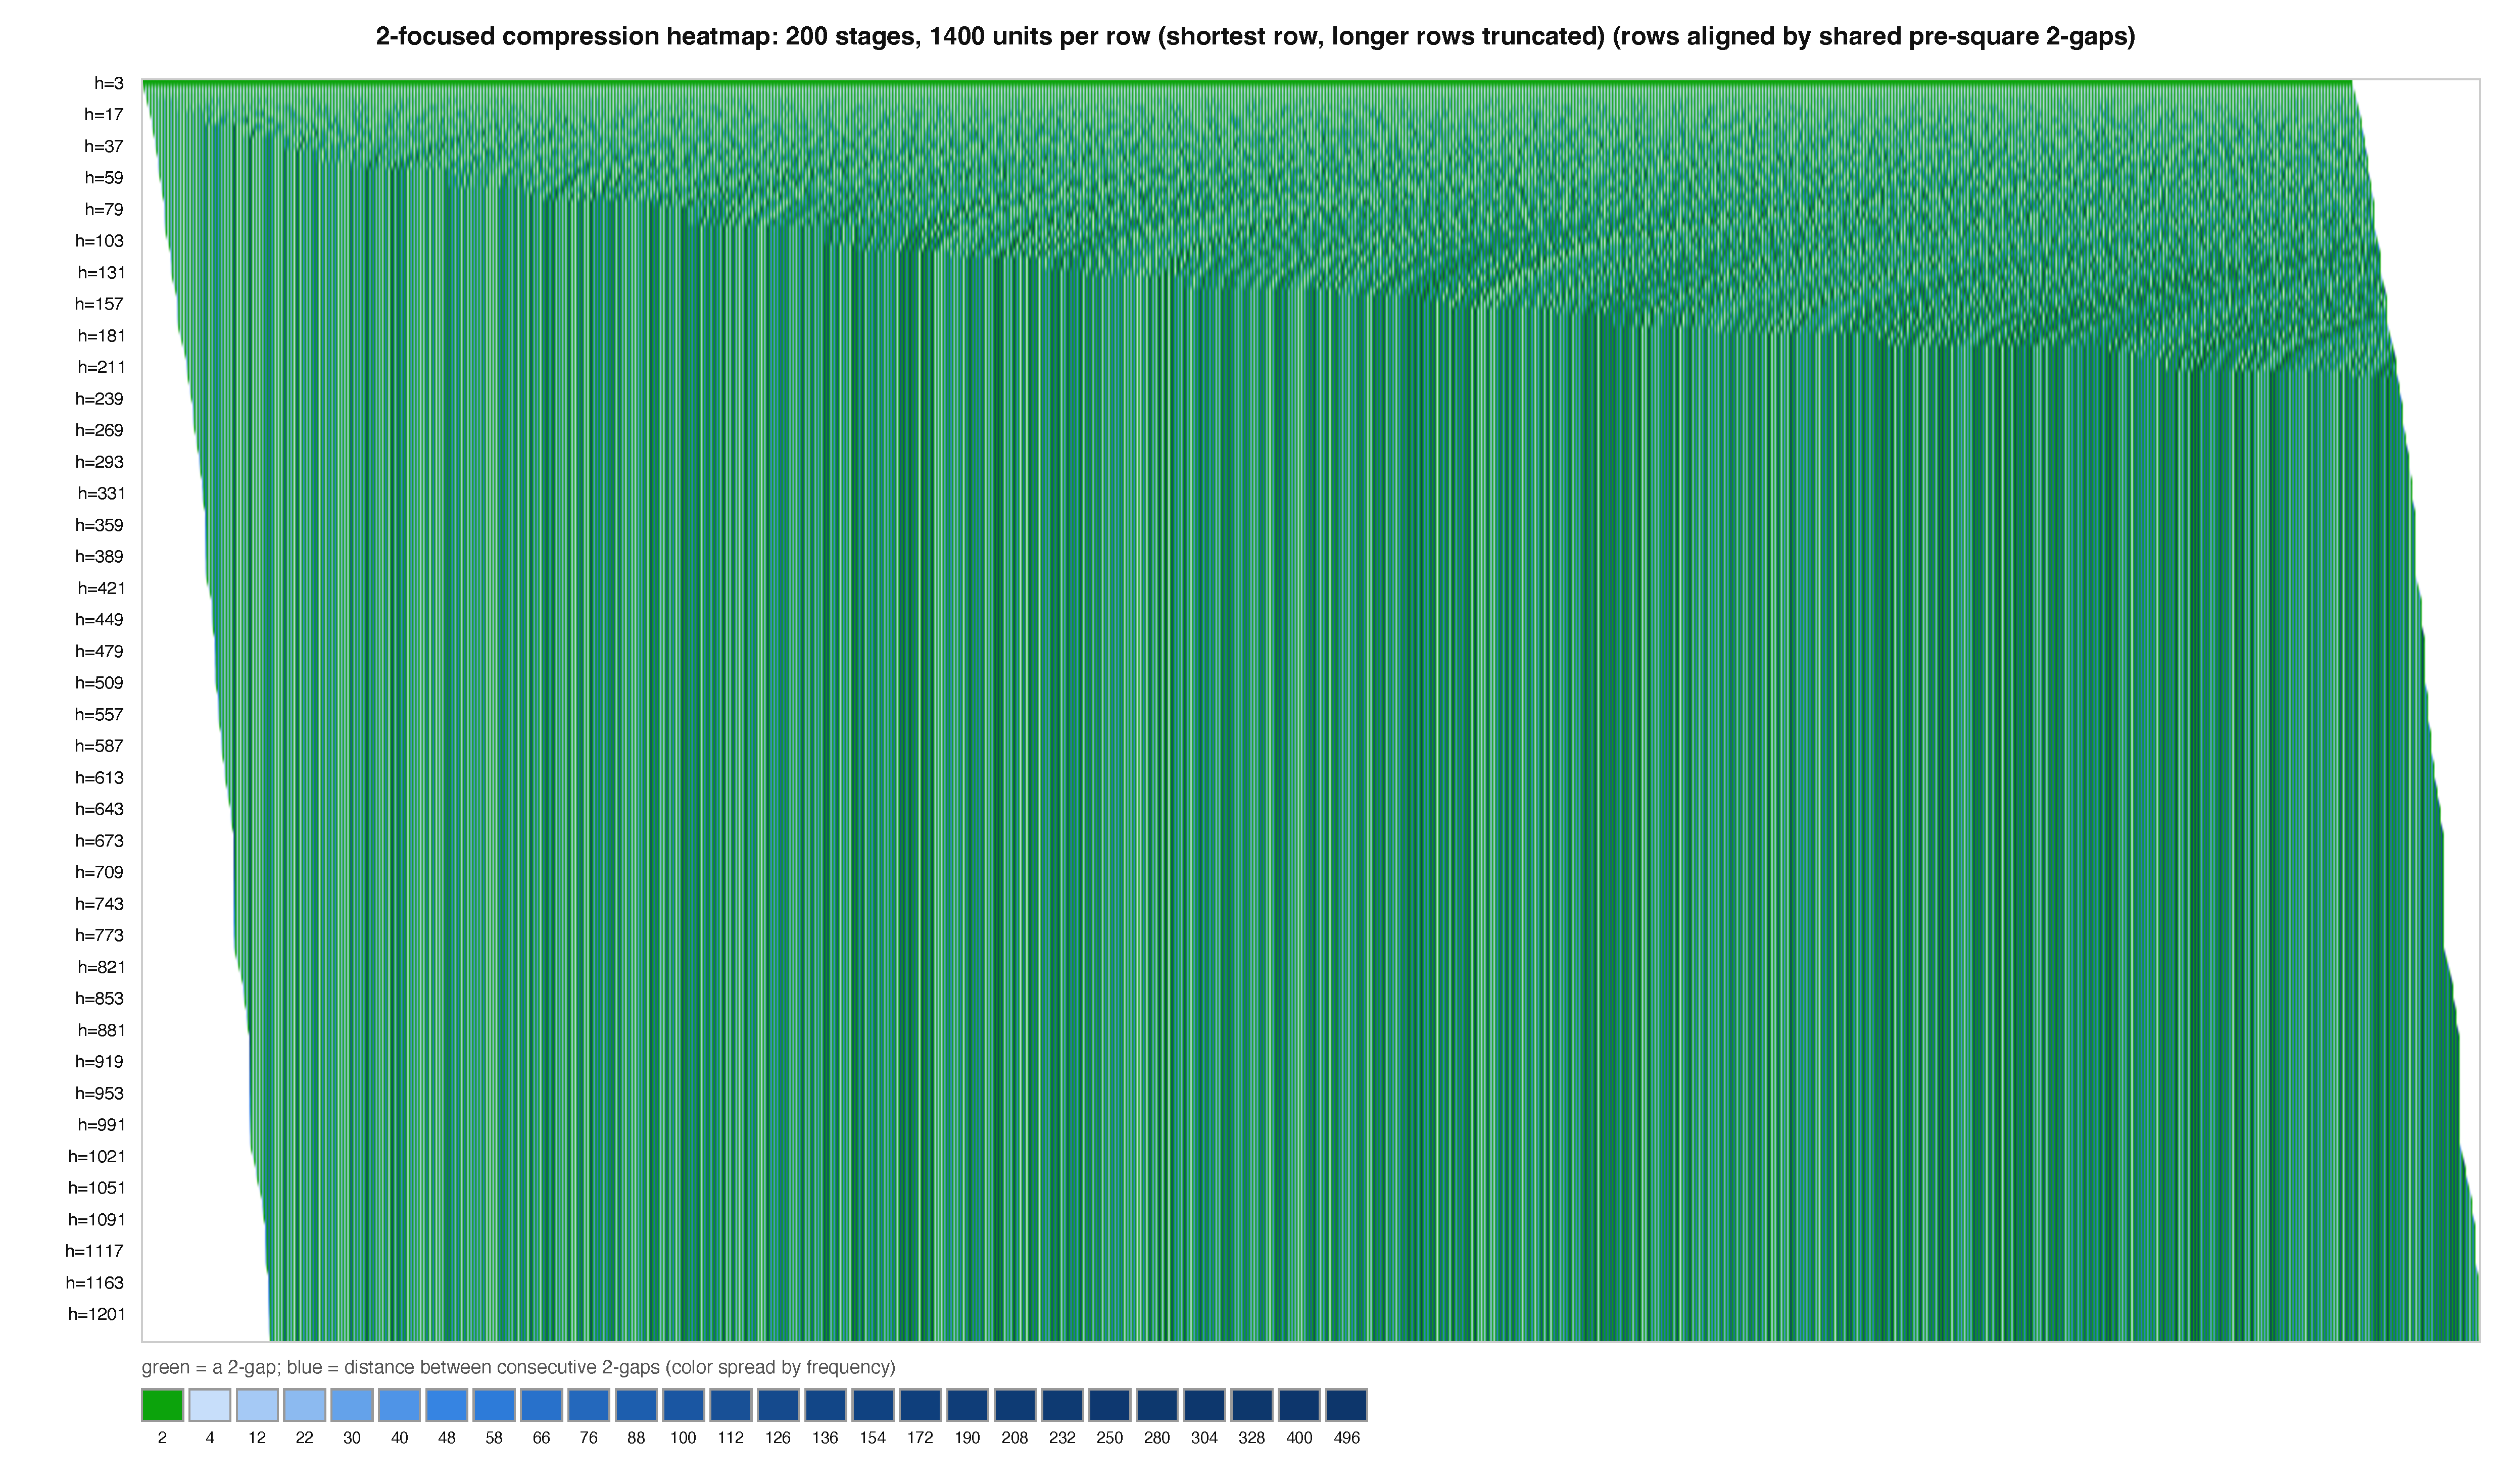
\includegraphics[width=\textwidth]{figures/gap-heatmap-2focused-aligned.pdf}
\caption{Shared-safe-2 aligned compression of 200 Sieve Sequence stages: unchanged pre-square 2-gaps form vertical green lines}
\end{figure}
The left white wedge is intentional padding created by the cumulative offsets. A zero shift occurs when advancing the head merely shortens the leading collapsed non-2 run; a one-cell shift occurs when that step removes an entire compressed run or a standalone 2-gap cell. Thus the straight green lines in View B and the curved texture in View A describe the same data under different coordinates.
The sieve does not rotate this compressed row as an atomic list. Within the safe prefix, it advances the head through one raw gap; only afterward does the visualization collapse the remaining consecutive non-2 gaps. Thus a raw prefix $[4,6,8,2,\ldots]$ appears over successive rows as $[18,2,\ldots] \to [14,2,\ldots] \to [8,2,\ldots] \to [2,\ldots]$. The long blue feature is not one unchanged merged gap reused in several sequences; it is the decreasing suffix of one raw run. Rotating one compressed cell per row would show that block only once, but it would define a different dynamics from the Sieve Sequence.
\begin{longtable}{@{}>{\raggedright\arraybackslash}p{0.14\textwidth}>{\raggedright\arraybackslash}p{0.32\textwidth}>{\raggedright\arraybackslash}p{0.44\textwidth}@{}}
\toprule
View & Horizontal coordinate & What vertical comparison supports \\
\midrule
Independent snapshots & Compressed units from each row's own head & Within-stage density and spacing texture; not cell-by-cell lineage \\
Shared-safe-2 aligned & Cumulative columns fixed by shared 2-gaps below the previous $h^2$ & Exact alignment of the observed safe prefix; not full lineage beyond it \\
\bottomrule
\end{longtable}
These figures provide empirical context for the placement problem; neither is evidence for the companion-model survival thresholds derived below. They are generated by the \href{https://github.com/thiagomata/prime-numbers/blob/master/python/src/sieve_sequence/gap_heatmap.py}{gap-heatmap calculation} from a dataset containing the \href{https://github.com/thiagomata/prime-numbers/blob/master/data/sieve-sequence/first_gaps_per_seq.csv}{first 100,000 gaps of each stage}.
The central question is therefore not what fixed percentage of behavior may be called adversarial. It is how large the realized local destruction may be relative to the random benchmark $2/r$, and how that damage is allocated near the head.
The balanced companions are designed to separate them. They retain the real sieve's exact number of descendants but replace the arithmetic rule selecting which descendants die. This makes global survival identical in every companion while allowing local behavior to range from maximally protective, through position-blind random, to maximally hostile.
We establish:
- the exact allocation-independent global recurrence $N_{k+1}=(r_k-2)N_k$; - the cumulative local-hazard law $P(Q)=e^{-D(Q)}$ and its fixed-factor and logarithmic survival frontiers; - the distinct square-window and head thresholds for adversarial/random and adversarial/protective mixtures; - sharp finite allocation bounds separating adversarial-label budget from positional information; and - exact-quota and biased exact-quota companions that preserve CRT strike counts while randomizing their locations.
\subsection{Scope and Evidence}
We prove exact identities for the finite companion processes and conditional theorems for their asymptotic local behavior. Whenever a result needs spatial uniformity, head availability, or cross-layer mixing, we state that premise in the property itself before using it. The comparison with the real sieve then shows what additional arithmetic information would transfer the companion result.
The companion theorems below are proved mathematically under their stated premises; Stainless verification remains pending and is outside this article's scope.
